\setcounter{section}{1}
\section{Methodology}


The benchmark is designed to be baseline for future applications that are using NanoVDB for narrow-band level-sets and raytracing within the context of Semiconductor process simulation.
Therefore no specific problem is chosen but the worst-case scenario in a typical application is modelled.

\subsection{Hardware setup}
The performance benchmark is performed on a single node of a scientific cluster provided by TU Wien.
The node consists of the devices listed in Tab. \ref{tab:hardware} which are both used for the benchmark.

CPUs and GPUs are different platforms in terms of architecture and design which makes a fair comparison with regards to their technical aspects difficult.
However both devices are similar in cost of acquisition and operating expenses (i.e. power usage).
Furthermore both platforms are marketed towards scientific computing.


\begin{table}[H]

	\caption{Hardware used for the benchmark. Prices may fluctuate due to current events. Power consumption represents the absolute maximum ratings according to the vendor}
	\centering
	\begin{tabular}{@{}llll@{}}
		\toprule
		                & Price           & Power Consumption & Cores                \\ \hline
		Intel Xeon 6248 & € 3.300         & 105W              & 20 Cores; 40 Threads \\
		NVIDIA Tesla T4 & € 2.500 - 3.000 & 70W               & 2.560 CUDA-Cores     \\ \bottomrule
	\end{tabular}
	\label{tab:hardware}
\end{table}


\subsection{Simulation environment}

A common problem in Semiconductor process simulation is light being cast into a trench with semi-reflective walls as shown in Fig. \ref{fig:benchmark_setup} (left).
To simplify the program and enforce a worst-case scenario the following modifications are performed:

\begin{itemize}
	\item Rays leaving the bounding box (i.e. shooting into the sky) are cheaper to compute but do not contribute to the simulation.
	      In order to prevent these edge cases rays are cast onto the inner surface of a hollow sphere.
	\item The point source is replaced with a volumetric source. Otherwise every ray would start within the same voxel which would lead to a beneficial memory access pattern.
	\item Depending on the reflecting angle, rays may cover different distances. Therefore the inner sphere (ray source) is offset to create a distribution of distances.
	\item Rays are shuffled in memory before being passed to the kernel to prevent beneficial memory access patterns.
	\item Any ray reflection on the surface is equivalent to having 2 separate rays (inbound and outbound) at the intersection point. Therefore reflections do not need to be modelled.
\end{itemize}


\begin{figure}[!htb]
	\minipage{0.32\textwidth}
	  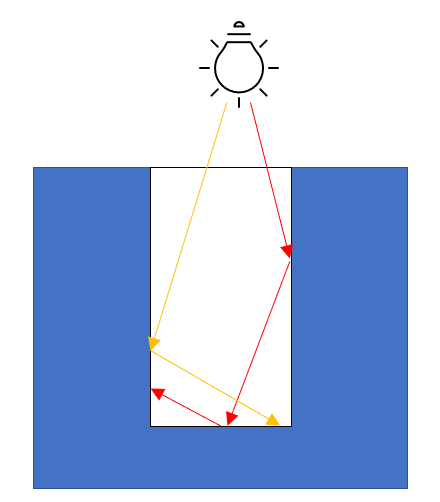
\includegraphics[width=\linewidth]{res/trench_with_rays.png}
	\endminipage\hfill
	\minipage{0.32\textwidth}
	  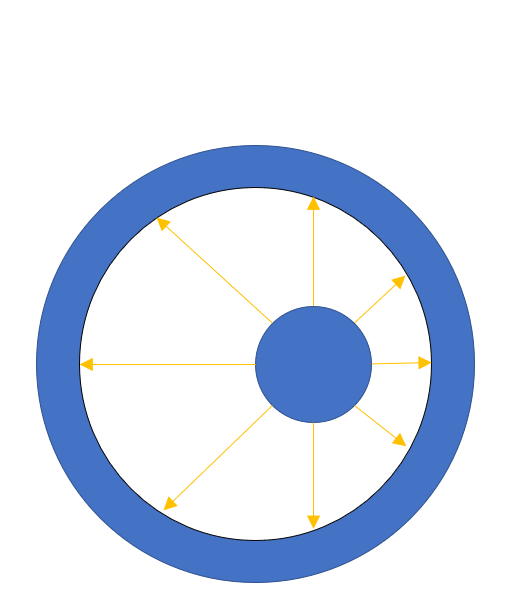
\includegraphics[width=\linewidth]{res/benchmark_setup.png}
	\endminipage\hfill
	\minipage{0.32\textwidth}
	  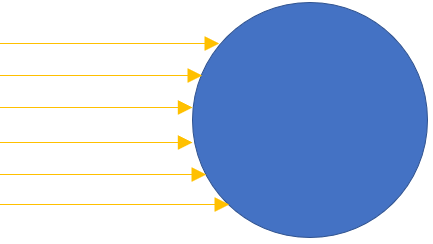
\includegraphics[width=\linewidth]{res/rays_on_sphere.png}
	\endminipage

		\caption{Benchmark setup. 
		\textbf{left} Trench being illuminated by a light source. Every ray has a chance of being reflected or absorbed.
		\textbf{center} 2D cross-section of the modified setup. 
		\textbf{right} Setup for determining accuracy of the calculation
		}
	\label{fig:benchmark_setup}
\end{figure}


Origin and direction of every ray along with a ground truth are precomputed and passed to three different ray intersection kernels:

\begin{itemize}
	\item OpenVDB (CPU)
	\item NanoVDB (CPU)
	\item NanoVDB (GPU)
\end{itemize}

The OpenVDB kernel servers as a baseline for comparison.
Both NanoVDB kernels are identical but launched on different platforms.

Only the time required to calculate intersections is measured. Memory management, data transfer, ray generation, result verification, etc. is not included.
After the benchmark is complete the number of calculated rays per second is derived using

\begin{equation}
	Rps = \frac{ray \: count}{time} = [\frac{1}{s}]
\end{equation}

The benchmark is repeated while increasing the number of rays until no further increases in $Rps$ is observed.
The asymptotic behaviour of the resulting performance curve is used to estimate a potential performance gain for switching to NanoVDB or GPUs.

After each iteration the resulting intersections ($\mathbf{r}_{calc}$) are compared to a pre-computed ground truth ($\mathbf{r}_{gt}$) to assure the correctness of the results. 
Results are considered correct if the following condition is satisfied for each ray:

\begin{equation}
	\lVert \mathbf{r}_{calc} - \mathbf{r}_{gt} \lVert _2 \:  \leq \sqrt{3} \cdot VOXEL\_SIZE
\end{equation}

In its current implementation NanoVDB only provides limited support for floating point calculations and  many functions only accept integer-based arguments.
Therefore NanoVDBs accuracy is investigated in an additional experiment using the setup shown in Fig. \ref{fig:benchmark_setup}c.
Parallel rays are projected onto a sphere and the resulting intersection points are compared to an analytical solution. 
The spacing between rays is set to be smaller than the voxel size. 

